
          %-----------------%
\chapter{~~Technical details}\label{\numb section 11}
          %-----------------%

Sections \ref{\numb section 11} and \ref{\numb section 12} are meant for those intereseted
in developing and extending \maniFEM.
Of course the ultimate documentation is the source code; these sections can be used as
a guide through the source code.


          %--------------------------%
\section{~~Namespaces and class names}\label{\numb section 11.\numb parag 1}
          %--------------------------%

All names in {\maniFEM} are wrapped into the namespace {\small\tt\verm{maniFEM}}.
We recommend {\small\tt using namespace \verm{maniFEM}} in your code,
otherwise the text will become cumbersome.
For instance, you will have to write {\small\tt\verm{maniFEM}::CellIterator} instead of
{\small\tt\verm{CellIterator}}, and so on.
We are {\small\tt using namespace \verm{maniFEM}} in the examples of this manual.

As a general rule, namespaces and class names are written with capital initial
letter$\;$:
{\small\tt\verm{Cell}}, {\small\tt\verm{Mesh}}, {\small\tt\verm{Integrator}},
{\small\tt\verm{FiniteElement}}, {\small\tt\verm{VariationalFormulation}}.
Namespace {\small\tt\verm{tag}} (see paragraph \ref{\numb section 11.\numb parag 3})
is an exception to the above rule.
Namespace {\small\tt\verm{maniFEM}} itself is also an exception, for merely aestetic reasons.

In \maniFEM, there are no {\small\tt private} or {\small\tt protected} class members or methods.
Everything is {\small\tt public};
the user can make use of any class member if he or she so chooses.
This can be considered poor design; we endorse this criticism with no further comments.

However, some class members and methods are intended to be used by the final user,
while others are used in the internal implementation of the former.
Classes \hbox{intended} for basic usage are directly exposed in {\small\tt namespace
\verm{maniFEM}}, for instance
{\small\tt\verm{Cell}}, {\small\tt\verm{Mesh}}, {\small\tt\verm{CellIterator}},
{\small\tt\verm{Function}}, {\small\tt\verm{Manifold}}, {\small\tt\verm{VariationalFormulation}},
{\small\tt\verm{Integrator}}, {\small\tt\verm{FiniteElement}}.
Classes not intended for the final user (at least not for the basic usage of \maniFEM)
have been hidden inside the above mentioned names, e.g. {\small\tt\verm{Mesh}::Positive},
\ {\small\tt\verm{CellIterator}::Over::SegsOfPosLoop::Positive},
\hbox{\small\tt\verm{Function}::CoupledWithField::Scalar}.
Also, in the source code there are comments like

\begin{Verbatim}[commandchars=\\\{\},formatcom=\small\tt,baselinestretch=0.94]
   \cinza{// do not use directly, let [some other method] do the job}
\end{Verbatim}

In an effort not to expose too many names in the {\small\tt\verm{maniFEM}} namespace, we have
used the namespace {\small\tt\verm{tag}::Util} to keep names which did not fit elsewhere.
We have also used anonymous namespaces in order to hide names of functions which are
only used in one file.

In the {\small\tt namespace \verm{maniFEM}} there are also many overloaded functions.
Because they take arguments of specific type, they will not clash with names defined
by the user.
Examples are : {\small\tt\verm{smooth\_\,min}}, {\small\tt\verm{power}}, {\small\tt\verm{abs}},
{\small\tt\verm{sin}}.


          %-------------%
\section{~~Code coloring}\label{\numb section 11.\numb parag 2}
          %-------------%

Throughout this manual, example {\tt C++} code is coloured according to the following
conventions.

Class names directly exposed in {\small\tt namespace \verm{maniFEM}} are shown in blue :
{\small\tt \verm{Cell}}, {\small\tt \verm{Mesh}}, {\small\tt \verm{CellIterator}},
{\small\tt \verm{Function}}, {\small\tt \verm{Manifold}},
{\small\tt \verm{VariationalFormulation}}, {\small\tt \verm{Integrator}},
{\small\tt \verm{FiniteElement}}, the rarely needed {\small\tt \verm{Field}} and
the even more rarely needed {\small\tt \verm{MeshIterator}} and {\small\tt\verm{MetricTree}}.
% There is an exception to this rule : the word {\small\tt tag}, although directly exposed
% in {\small\tt namespace \verm{maniFEM}}, is not coloured
% (that's because we want it to be discrete).
There are also functions like {\small\tt \verm{smooth\_\,min}} and also overloaded versions
of common functions like {\small\tt\verm{power}}, {\small\tt \verm{sin}}, {\small\tt \verm{cos}}.

Newly declared objects are shown in \azul{purple}.

Comments are \cinza{grey}.

Strings are \verde{dark green}.


          %----%
\section{~~Tags}\label{\numb section 11.\numb parag 3}
          %----%

We use extensively {\small\tt\verm{tag}}s.
These are {\tt C++} structures gathered in the {\small\tt namespace \verm{tag}}.
Most of them contain no data; only their type is useful, at compile time.

A {\small\tt\verm{tag}} is used to clearly distinguish between functions with the same name
(overloaded functions).
For instance, in the code excerpt below five {\small\tt\verm{CellIterator}}s are defined
by means of different (overloaded) methods having the same name {\small\tt\verm{Mesh}::iterator});
the iterators behave very differently (see paragraphs \ref{\numb section 9.\numb parag 5} and
\ref{\numb section 9.\numb parag 6}).

\begin{Verbatim}[commandchars=\\\{\},formatcom=\small\tt,baselinestretch=0.94]
   \cinza{// 'chain' is a one-dimensional Mesh}
   \verm{CellIterator} \azul{it1} = chain.iterator ( \verm{tag}::over_vertices );
   \verm{CellIterator} \azul{it2} = chain.iterator ( \verm{tag}::over_vertices, \verm{tag}::backwards );
   \verm{CellIterator} \azul{it3} = chain.iterator ( \verm{tag}::over_segments );
   \verm{CellIterator} \azul{it4} = chain.iterator ( \verm{tag}::over_segments, \verm{tag}::backwards );
   \verm{CellIterator} \azul{it5} = chain.iterator ( \verm{tag}::over_segments, \verm{tag}::force_positive );
\end{Verbatim}

The above could be achieved by giving longer names to the functions, but we believe
{\small\tt\verm{tag}}s make the code more readable.
Besides that, in the case of constructors, we do not have the choice of the name of the function
(a constructor has the same name as its class).
{\ManiFEM} uses {\small\tt\verm{tag}}s extensively for constructors, e.g.
\begin{Verbatim}[commandchars=\\\{\},formatcom=\small\tt,baselinestretch=0.94]
   \verm{Cell} \azul{A} ( \verm{tag}::vertex );  \verm{Cell} \azul{B} ( \verm{tag}::vertex );
   \verm{Mesh} \azul{AB} ( \verm{tag}::segment, A.reverse(), B, \verm{tag}::divided_in, 10 );
\end{Verbatim}

In \maniFEM, namespaces and class names begin with capital letter
(see paragraph \ref{\numb section 11.\numb parag 1})
The namespace {\small\tt\verm{tag}} (or {\small\tt \verm{maniFEM}::tag} if you are not
{\small\tt using namespace \verm{maniFEM}}) is an exception to the above rule.
We prefer its name to have only lower case letters because we want it to be
discrete. For instance, if we wrote {\small\tt\verm{Tag}::divided\_\,in},
the reader's eye would catch {\small\tt\verm{Tag}} much before {\small\tt divided\_\,in};
thus, {\small\tt\verm{tag}::divided\_\,in} is more readable.
Of course, the final user has the choice of {\small\tt using namespace \verm{tag}}
but beware, it has many names which may conflict with the ones in your code.

Most tags have only lower-case letters and underscores.
The exceptions are proper names : {\small\tt \verm{tag}::Lagrange}, {\small\tt \verm{tag}::Euclid}.


          %------------------%
\section{~~Wrappers and cores}\label{\numb section 11.\numb parag 4}
          %------------------%

Designing and implementing {\maniFEM} has been a challenging endeavour.
We had a lot of fun and we have learned much along the process.

Take cells and meshes, for instance.
As explained in paragraph \ref{\numb section 1.\numb parag 2}, at the conceptual level meshes
are roughly collections of cells of the same dimension and cells are essentially
defined by their boundary which is a lower-dimensional mesh.
This conceptual simplicity does not survive to the demands of an efficient code
(although it has been extremely useful in the process of designing \maniFEM;
it should also be useful for learning and using it).

Vertices (zero-dimensional cells) have no boundary at all.
One-dimensional cells (segments) have all the same shape and have a rudimentary boundary
(a zero-dimensional mesh consisting of a {\small\tt base} and a {\small\tt tip}).
In order to save space in the computer's memory, specific classes have been created for
vertices and for segments.

Also, there are positive cells and negative cells, positive meshes and negative meshes.
A positive cell and its negative counterpart (its {\small\tt reverse}) share some information.
To save memory space, negative cells are implemented in different classes from
positive cells, thus avoiding the storage of some of the redundant information.

We want, however, to manipulate all these different cells through a uniform interface,
which is where {\tt C++}'s inheritance and polymorphishm mechanisms come handy.
Thus, there are classes {\small\tt\verm{Cell}::Positive::Vertex},
{\small\tt\verm{Cell}::Positive::Segment} and {\small\tt\verm{Cell}::Positive::HighDim},
all derived from {\small\tt\verm{Cell}::Positive}.
And we have {\small\tt\verm{Cell}::Negative::Vertex},
{\small\tt\verm{Cell}::Negative::Segment} and {\small\tt\verm{Cell}::Negative::HighDim},
all derived from {\small\tt\verm{Cell}::Negative}.
Both {\small\tt\verm{Cell}::Positive} and {\small\tt\verm{Cell}::Negative} are derived from
{\small\tt\verm{Cell}::Core}.
% See the graph in figure \ref{\numb section 11.\numb fig 1}.
The graph below shows these inheritance relations; dotted lines represent relations subject to
the {\small\tt -DMANIFEM\_\,COLLECT\_\,CM} compilation option, explained in paragraph
\ref{\numb section 11.\numb parag 5}.

\begin{figure}[ht] \centering
 \psfrag{tag::Util::Core::Inactive}{{\small\tt\verm{tag}::Util::Core::Inactive}}
 \psfrag{tag::Util::Core::DelegateDispose}{{\small\tt\verm{tag}::Util::Core::DelegateDispose}}
 \psfrag{tag::Util::Core}{{\small\tt\verm{tag}::Util::Core}}
 \psfrag{Cell::Core}{{\small\tt\verm{Cell}::Core}}
 \psfrag{Cell::Negative}{{\small\tt\verm{Cell}::Negative}}
 \psfrag{Cell::Positive}{{\small\tt\verm{Cell}::Positive}}
 \psfrag{Cell::Negative::Vertex}{{\small\tt\verm{Cell}::Negative::Vertex}}
 \psfrag{Cell::Negative::NotVertex}{{\small\tt\verm{Cell}::Negative::NotVertex}}
 \psfrag{Cell::Positive::Vertex}{{\small\tt\verm{Cell}::Positive::Vertex}}
 \psfrag{Cell::Positive::NotVertex}{{\small\tt\verm{Cell}::Positive::NotVertex}}
 \psfrag{Cell::Negative::HighDim}{{\small\tt\verm{Cell}::Negative::HighDim}}
 \psfrag{Cell::Positive::HighDim}{{\small\tt\verm{Cell}::Positive::HighDim}}
 \psfrag{Cell::Negative::Segment}{{\small\tt\verm{Cell}::Negative::Segment}}
 \psfrag{Cell::Positive::Segment}{{\small\tt\verm{Cell}::Positive::Segment}}
 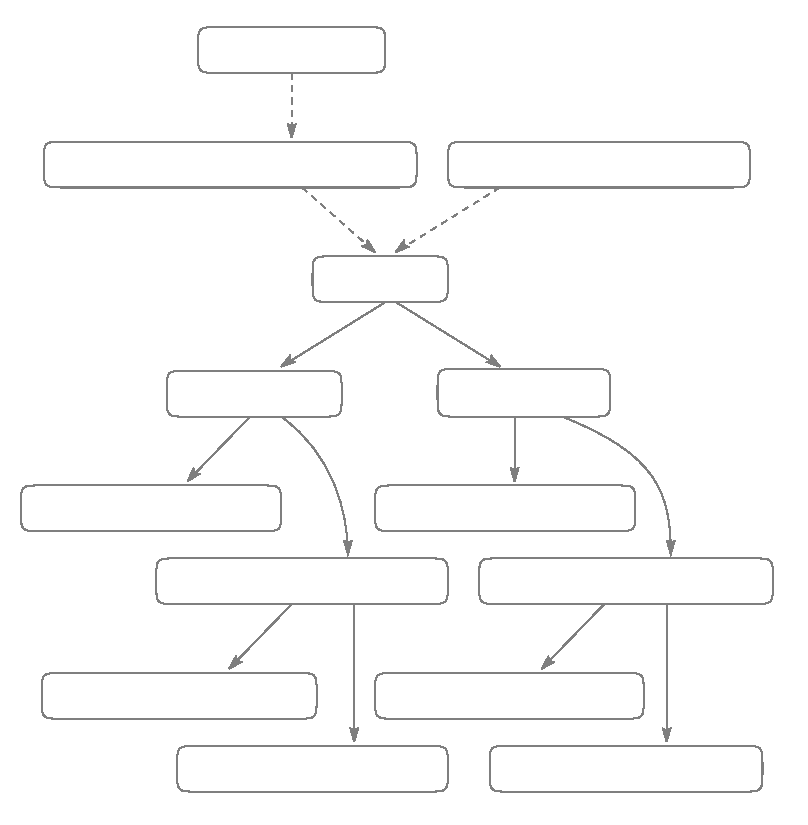
\includegraphics{diagr-cell-rev}
 \caption{Inheritance diagram for {\small\tt\verm{Cell}} cores}
 \label{\numb section 11.\numb fig 1}
\end{figure}

On the other hand, we want cells and meshes to be persistent objects (not subject to
syntactic scope).
We create them within some function and we want them to remain alive after returning
to the main program.
Also, they are unique entities, it does not make sense to copy them.
This is why we have implemented {\small\tt \verm{Cell}} as a thin wrapper around
{\small\tt \verm{Cell}::Core}
with most methods of {\small\tt \verm{Cell}} being delegated to {\small\tt \verm{Cell}::Core}.
When it goes out of its syntactic scope, the wrapper is destroyed but the {\small\tt \verm{Cell}::Core}
object inside remains intact (unless there are no more wrappers for that core, as explained in
paragraph \ref{\numb section 11.\numb parag 5}).
Also, you can copy the wrapper as in {\small\tt \verm{Cell} A = B} or {\small\tt \verm{Mesh} BA = AB.reverse()}
but these operations do not create new core objects, they just give new names to
already existing cells or meshes (paragraph \ref{\numb section 9.\numb parag 12} gives
more details).
You can think of {\small\tt \verm{Cell}}s and {\small\tt \verm{Mesh}}es as customized pointers towards
{\small\tt \verm{Cell}::Core}s and {\small\tt \verm{Mesh}::Core}s, respectively.

Negative meshes contain no useful information; they appear mostly as boundaries
of negative cells, sometimes as interfaces between subdomains of our mesh.
Thus, there is no such class as {\small\tt \verm{Mesh}::Negative};
all {\small\tt \verm{Mesh}::Core}s are positive.
The wrapper class {\small\tt \verm{Mesh}} contains a pointer to a {\small\tt \verm{Mesh}::Core}
and a flag telling it to reverse everything if the mesh is to be considered negative.
Zero-dimensional meshes (boundaries of segments) are not stored at all.
One-dimensional meshes have often a particular structure (they are chains of segments);
when this happens they are implemented in a specialized class {\small\tt \verm{Mesh}::Connected::OneDim}.
% See the graph in figure \ref{\numb section 11.\numb fig 2}.
The graph below shows these inheritance relations; dotted lines represent relations subject to
the {\small\tt -DMANIFEM\_\,COLLECT\_\,CM} compilation option, explained in paragraph
\ref{\numb section 11.\numb parag 5}.

\begin{figure}[ht] \centering
 \psfrag{tag::Util::Core}{{\small\tt\verm{tag}::Util::Core}}
 \psfrag{Mesh::Core}{{\small\tt\verm{Mesh}::Core}}
 \psfrag{Mesh::NotZeroDim}{{\small\tt\verm{Mesh}::NotZeroDim}}
 \psfrag{Mesh::ZeroDim}{{\small\tt\verm{Mesh}::ZeroDim}}
 \psfrag{Mesh::Fuzzy}{{\small\tt\verm{Mesh}::Fuzzy}}
 \psfrag{Mesh::STSI}{{\small\tt\verm{Mesh}::STSI}}
 \psfrag{Mesh::Connected::OneDim}{{\small\tt\verm{Mesh}::Connected::OneDim}}
 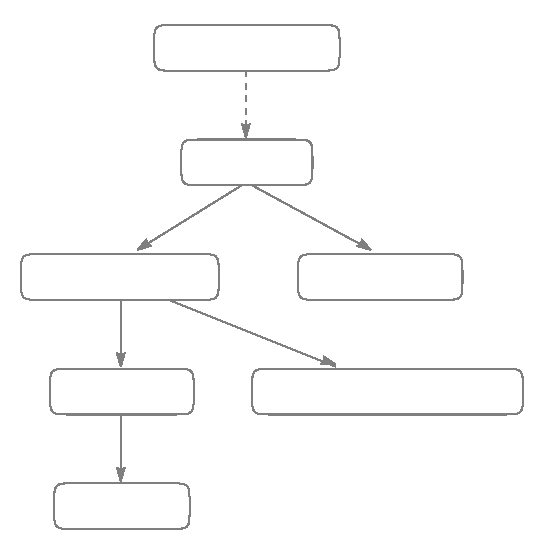
\includegraphics{diagr-mesh-rev}
 \caption{Inheritance diagram for {\small\tt\verm{Mesh}} cores}
 \label{\numb section 11.\numb fig 2}
\end{figure}

To save memory, we don't even keep the dimension of a cell as an attribute,
it's a static property for vertices and segments, while for higher-dimensional cells
it's obtained from the boundary's dimension.
The dimension of a mesh is not kept as an attribute either; it's computed on-the-fly
by counting the levels of collections of cells the mesh is made of (and then
substracting one).
For instance, the mesh in paragraph \ref{\numb section 1.\numb parag 1} has three layers
of cells : points, segments and squares.

Constructors for wrapper classes act as factory functions for the core object.
According to their arguments, they build different core objects.

Other objects have been implemented using the same logic of wrappers and core objects :
iterators, fields, functions, manifolds.

% There are Euclidian manifolds, cartesian products, implicitly defined submanifolds and
% parametrized submanifolds.
% Distinct notions with very different internal implementations.
% But we would like to offer the user the possibility of declaring any of these as ``a
% {\small\tt Manifold}''.
\vfil\break


          %------------------------%
\section{~~The lifecycle of objects}\label{\numb section 11.\numb parag 5}
          %------------------------%

Many objects in {\maniFEM} are implemented using a wrapper-core model.
Examples are {\small\tt\verm{Cell}}s, {\small\tt\verm{Mesh}}es,
{\small\tt\verm{CellIterator}}s, {\small\tt\verm{MeshIterator}}s, {\small\tt\verm{Manifold}}s,
{\small\tt\verm{Function}}s, {\small\tt\verm{FiniteElement}}s, {\small\tt\verm{Integrator}}s,%
\break {\small\tt\verm{VariationalFormulation}}s.
A garbage collector is implemented; all these classes inherit from
{\small\tt \verm{tag}::Util::Wrapper} and
their cores inherit from {\small\tt \verm{tag}::Util::Core}.
Wrappers contain a pointer to a core; each core keeps a counter of wrappers pointing to it.
The destructor of a wrapper decrements the counter and destroys the core if the counter
reaches zero.
It's like a {\small\tt shared\_\,ptr}.

Cells and meshes depend on each other in a complicated manner.
A cell keeps its boundary (which is a mesh) alive.
A mesh keeps its component cells alive.
A negative cell keeps alive its positive counterpart but the reverse does not hold;
care must be taken to break dependency cycles.

Some programs consist only in building a mesh and never (or rarely) discarding cells.
For such programs, there is no advantage in using a {\small\tt shared\_\,ptr}-like strategy.
Thus, unlike for other {\maniFEM} objects, the garbage collector for {\small\tt \verm{Cell}}s and
{\small\tt \verm{Mesh}}es can be turned off by erasing the option
{\small\tt -DMANIFEM\_\,COLLECT\_\,CM} in the {\small\tt Makefile}.
Remember to {\small\tt make clean} and re-build your program;
see also paragraph \ref{\numb section 11.\numb parag 15}.
The graphs in figures \ref{\numb section 11.\numb fig 1} and \ref{\numb section 11.\numb fig 2}
show dotted lines where the inheritance relationship is subject to the
{\small\tt -DMANIFEM\_\,COLLECT\_\,CM} option.
If you turn off the garbage collector, {\small\tt \verm{Cell}}s and {\small\tt \verm{Mesh}}es
will occupy less space in the computer's memory and your program will run slightly faster.
However you should not turn it off if you do a lot of remeshing,
or ghost cells and meshes will fill the computer's memory (this is known as ``memory leak'').

In some examples, the garbage collector for cells and meshes does not work well :
the cell counter does not reach zero, as it should, at the end of the program.
In some cases, this happens because the finite elements are not properly destroyed.
In other cases, it has to do with the {\small\tt\verm{MetricTree}} (described in
paragraph \ref{\numb section 12.\numb parag 10}) which is not properly cleaned.


          %-------------------------%
\section{~~Different kinds of meshes}\label{\numb section 11.\numb parag 6}   
          %-------------------------%

A {\small\tt \verm{Mesh}} wrapper contains a pointer to a {\small\tt \verm{Mesh}::Core}.
The latter is a polymorphic object; there are several different kinds of meshes
which differ in their internal implementation; the wrapper provides a uniform interface
to the user (making use of virtual methods of the core).

Negative meshes are temporary wrappers built on-the-fly.
Their core points to a positive mesh.

Zero-dimensional meshes appear only as boundaries of segment {\small\tt \verm{Cell}}s.
They are temporary objects built on-the-fly.

Some meshes are implemented as {\small\tt \verm{Mesh}::Fuzzy}.
They have as attributes lists of cells of different dimensions;
these lists have no particular order.
Iterators over cells of {\small\tt Fuzzy} meshes simply run over the respective lists of cells.

Other meshes are assumed to be connected and keep no lists of cells.
Iterators over such meshes traverse the mesh beginning at a starting point (which is an attribute
of class {\small\tt \verm{Mesh}:: ::Connected::***Dim}) and then using the neighbourhood relations
to move from one cell to another.

One-dimensional connected meshes are a special case because their topology is peculiar;
segments and vertices composing such a mesh have a natural order (linear order).
Recall that all meshes in {\maniFEM} are oriented.
A one-dimensional connected mesh can be a closed loop or an open chain of segments.
In the latter case, there is a natural starting point (the first vertex or first segment).
Iterators over such meshes are described in paragraph \ref{\numb section 9.\numb parag 6}.
The {\small\tt \verm{Mesh}} constructor with {\small\tt \verm{tag}::segment} builds an open
{\small\tt \verm{Mesh}::Connected::OneDim}.
Also, cell constructors with {\small\tt \verm{tag}::triangle} and {\small\tt \verm{tag}::quadrangle} produce cells
whose boundary is a closed {\small\tt \verm{Mesh}::Connected::OneDim}.

Connected meshes of dimension two or higher are not yet implemented; for now,
{\small\tt \verm{Mesh}} constructors with {\small\tt \verm{tag}::rectange} or
{\small\tt \verm{tag}::triangle} build a {\small\tt Fuzzy} mesh instead.
A class {\small\tt \verm{Mesh}::Connected:: ::HighDim} is object of current work.
We also intend to implement multiply connected meshes.

{\small\tt STSI} meshes are object of current work (see the graph in figure
\ref{\numb section 11.\numb fig 2}); the name means ``self-touching or self-intersecting'' meshes.
They will be used internally to implement iterators over connected high-dimensional meshes,
and for progressive meshing (described in section \ref{\numb section 3}).

Iterators over cells of a {\small\tt Fuzzy} mesh are fast because they simply run over the
list of cells of given dimension.
Iterators over {\small\tt Connected} meshes may be slower because they traverse the mesh using
neighbourhood relations between cells.
On the other hand, {\small\tt Fuzzy} meshes require more space in the computer's memory.

The kind of a certain mesh is not always completely obvious.
For instance, when {\small\tt join}ing two meshes of the kind
{\small\tt \verm{Mesh}::Connected::OneDim}, the result will be a
{\small\tt \verm{Mesh}::Connected::OneDim} if the last vertex of one of the meshes
is the same as the first vertex (reversed) of the other mesh.
Otherwise, the result will be a {\small\tt \verm{Mesh}::Fuzzy}.


          %-----------------------------%
\section{~~Maximum topological dimension}\label{\numb section 11.\numb parag 7}
          %-----------------------------%

\leavevmode {\ManiFEM} assumes you will not build meshes of topological dimension
above 3.
If you want to play with higher-dimensional meshes, you must relax this assumption
through the statement {\small\tt \verm{Mesh}::set\_\,max\_\,dim (}some-integer{\small\tt )}.

On the other hand, you may want to decrease the expected dimension.
Suppose you want to mesh surfaces in $ \mathbb{R}^3 $.
This means your maximum topological dimension will be 2
(this has nothing to do with the geometric dimension, here 3).
Then you may state your intention at the beginning of your program
(before building any cell, before even declaring the first vertex) through
the statement {\small\tt \verm{Mesh}::set\_\,max\_\,dim(2)}.
This will decrease the size of the {\small\tt \verm{Cell}::Core} objects in your code,
thus saving some memory.

But beware, if you try to build a mesh of dimension higher than the one expected by
\maniFEM, you will get an {\small\tt assertion error} at run-time in {\small\tt DEBUG} mode,
or some bizarre behaviour (often a {\small\tt segmentation fault}) in {\small\tt NDEBUG} mode.
The {\small\tt DEBUG} mode is explained in paragraph \ref{\numb section 11.\numb parag 15}.

The geometric dimension is set by simply declaring a Euclidian manifold and building
a coordinate system on it (see e.g.\ paragraphs \ref{\numb section 1.\numb parag 1}
and \ref{\numb section 2.\numb parag 16}).


          %--------------------%
\section{~~Cores of cells and meshes}\label{\numb section 11.\numb parag 8}
          %--------------------%

As explained in paragraph \ref{\numb section 11.\numb parag 4}, the {\small\tt \verm{Cell}}
class is just a thin wrapper around a {\small\tt \verm{Cell}::Core}.
While it is possible and useful to copy {\small\tt \verm{Cell}}s (think of them as customized
pointers to {\small\tt \verm{Cell}::Core}s), objects in the {\small\tt \verm{Cell}::Core}
class cannot be copied.
Similarly, {\small\tt \verm{Mesh}} objects (wrappers) are customized pointers towards
{\small\tt \verm{Mesh}::Core}s; the latter cannot be copied.

The following classes of core cells are abstract and cannot be instantiated :
{\small\tt \verm{Cell}::Core}, {\small\tt \verm{Cell}::Positive},
{\small\tt \verm{Cell}::Core::Negative}, {\small\tt \verm{Cell}::Positive::NotVertex},
{\small\tt \verm{Cell}::Negative::NotVertex}.

The following classes of core cells can be instantiated :
{\small\tt \verm{Cell}::Positive::Vertex}, {\small\tt \verm{Cell}::Negative:: ::Vertex},
{\small\tt \verm{Cell}::Positive::Segment}, {\small\tt \verm{Cell}::Negative::Segment},
{\small\tt \verm{Cell}::Positive::HighDim},\break
{\small\tt \verm{Cell}::Negative::HighDim}.

Classes {\small\tt \verm{Mesh}::Core} and {\small\tt \verm{Mesh}::NotZeroDim} are abstract
and cannot be instatiated.

Classes {\small\tt \verm{Mesh}::ZeroDim}, {\small\tt \verm{Mesh}::Connected::OneDim} and
{\small\tt \verm{Mesh}::Fuzzy} can be instantiated.
Classes {\small\tt \verm{Mesh}::MultiplyConnected::OneDim},
{\small\tt \verm{Mesh}::Connected::HighDim}, {\small\tt \verm{Mesh}::MultiplyConneted::HighDim}
and {\small\tt \verm{Mesh}::STSI} are object of on-going work.

Note that there are no negative mesh cores.

The graphs in figures \ref{\numb section 11.\numb fig 1} and \ref{\numb section 11.\numb fig 2}
show inheritance relationships between these classes; dotted lines represent
inheritance relationships  subject to the {\small\tt -DMANIFEM\_\,COLLECT\_\,CM} option.


          %----------------------------------%
\section{~~Adding and removing cells or faces}\label{\numb section 11.\numb parag 9}
          %----------------------------------%

At a high level, we build cells and meshes using the appropriate {\small\tt \verm{Cell}} and
{\small\tt \verm{Mesh}} constructors.
At low level, cells and meshes are built by methods {\small\tt \verm{Cell}::glue\_\,on\_\,bdry\_\,of},
{\small\tt \verm{Cell}::cut\_\,from\_\,bdry\_\,of}, {\small\tt \verm{Cell}::add\_\,to\_\,mesh} and
{\small\tt \verm{Cell}::remove\_\,from\_\,mesh}.

The inlined method {\small\tt \verm{Cell}::glue\_\,on\_\,bdry\_\,of} is used for sticking a new
{\small\tt face} on the
boundary of an existing cell {\small\tt cll} (whose boundary is incomplete).
It simply calls the inlined method \ {\small\tt \verm{Cell}::Core::glue\_\,on\_\,bdry\_\,of}
which in turn calls the virtual method {\small\tt cll->glue\_\,on\_\,my\_\,bdry(face)}.
Different methods {\small\tt \verm{Cell}::***::glue\_\,on\_\,my\_\,bdry} exist for different kinds of
cells but to summarize we state that {\small\tt glue\_\,on\_\,my\_\,bdry} first calls
{\small\tt face->add\_\,to\_\,bdry} in order to add the face to the boundary of {\small\tt cll}
then calls the inlined method {\small\tt \verm{Cell}::Positive::NotVertex::glue\_\,common}.

Method {\small\tt \verm{Cell}::Core::add\_\,to\_\,bdry} is virtual so it does different things for
different kinds of cells but the common idea is that it calls another virtual method
{\small\tt \verm{Mesh}::Core::add\_\,***} (the name depends on the type of cell being added).
The latter calls an inline function {\small\tt make\_\,deep\_\,connections} (hidden in an anonymous
namespace in {\small\tt mesh.cpp}) which updates fields
{\small\tt \verm{Cell}::Positive::meshes}, {\small\tt \verm{Cell}::Positive***::meshes\_\,same\_\,dim} and
{\small\tt \verm{Mesh}::Fuzzy::cells} for several pairs cell-mesh
(including cells of lower dimension and meshes of higher dimension).
After that, {\small\tt \verm{Mesh}::Core::add\_\,***} updates neighbourhood relations
coded in the map {\small\tt \verm{Cell}::Core:: ::cell\_\,behind\_\,within}.

The inlined method {\small\tt \verm{Cell}::Positive::NotVertex::glue\_\,common} deals with
the case when the cell (on whose boundary we are trying to glue a new face)
already belongs to some mesh(es).
In that case, it updates the information in {\small\tt face->cell\_\,behind\_\,within}.

If we want to add a cell to a mesh which is not a boundary of a cell (this happens
frequently in {\small\tt \verm{Mesh}} constructors),
we call the inlined method {\small\tt \verm{Cell}::add\_\,to} which calls the virtual method
{\small\tt \verm{Cell}::Core::add\_\,to\_\,mesh} which is similar to {\small\tt \verm{Cell}::Core::add\_\,to\_\,bdry}
described above.

In the constructor of a cell, since we are sure there are no meshes containing that cell
(the cell is just being built),
we call method {\small\tt add\_\,to\_\,mesh} instead of {\small\tt glue\_\,on\_\,bdry\_\,of}
(we pretend the mesh is not a boundary).

Removing a face from the boundary of an existing cell, or removing a cell from a mesh
which is not a boundary, implies a process similar to the one described above,
with methods replaced by {\small\tt \verm{Cell}::cut\_\,from\_\,bdry\_\,of},
{\small\tt \verm{Cell}::remove\_\,from\_\,mesh},
{\small\tt \verm{Cell}::Core::cut\_\,from\_\,bdry\_\,of},
{\small\tt \verm{Cell}::Core::cut\_\,from\_\,my\_\,bdry},
{\small\tt \verm{Cell}::Core::remove\_\,from\_\,bdry}, {\small\tt \verm{Cell}::Core::remove\_\,from\_\,mesh},
{\small\tt \verm{Mesh}::Core:remove\_\,***}, {\small\tt break\_\,deep\_\,connections},
{\small\tt \verm{Cell}::Positive::NotVertex::cut\_\,common}.


                 %----------------------%
\section{~~\cinza{About {\tt init\_\,cell}} (outdated)}\label{\numb section 11.\numb parag 10}
                 %----------------------%

The {\small\tt \verm{Cell}} class has static attributes {\small\tt init\_\,cell},
{\small\tt init\_\,cell\_\,r}, {\small\tt data\_\,for\_\,init}, {\small\tt data\_\,for\_\,init\_\,r}.
The attribute {\small\tt init\_\,cell} is a list of pointers to functions to be called by
the constructor of a positive cell, while {\small\tt data\_\,for\_\,init} is a void pointer which
can be used to pass supplementary information to {\small\tt init\_\,cell}.
Attributes {\small\tt init\_\,cell\_\,r} and {\small\tt data\_\,for\_\,init\_\,r} fulfill a similar task
when building negative cells.

For instance, {\small\tt \verm{Manifold}::coordinate\_\,system} inserts into the list
{\small\tt \verm{Cell}::init\_\,cell[0]} a call to {\small\tt \verm{Mesh}::prescribe\_\,on} which in turn calls
{\small\tt \verm{FunctionOnMesh}::prescribe\_\,on} in order to prepare the ground for instructions like
{\small\tt \azul{x} == 1.0} to produce the desired effect after the creation of each point.

Another example is the constructor {\small\tt\verm{FiniteElement}::Lagrange::Q1} which
adds a call to\break {\small\tt\verm{FiniteElement}::Lagrange::Q1::enumerate\_\;new\_\,vertex} to
the list {\small\tt\verm{Cell}::init\_\,cell[0]}.
This way, future vertices will receive automatically a {\small\tt size\_\,t} label, to be used
by Lagrange finite elements.


\section{~~\cinza{[empty]}}\label{\numb section 11.\numb parag 11}


          %-----------------%
\section{~~Programming style}\label{\numb section 11.\numb parag 12}
          %-----------------%

I (Cristian) have chosen some program-writing conventions which may seem unusual for some people.
For instance, most programmers use braces like this

\begin{Verbatim}[commandchars=\\\{\},formatcom=\small\tt,baselinestretch=0.94]
   for ( ... ) \{
      statement 1;
      statement 2;
      statement 3;
   \}
\end{Verbatim}

or perhaps like this

\begin{Verbatim}[commandchars=\\\{\},formatcom=\small\tt,baselinestretch=0.94]
   for ( ... )
   \{
      statement 1;
      statement 2;
      statement 3;
   \}
\end{Verbatim}

I just can't accept the idea that a brace opens more to the right than it closes, or at the
same point.
For me, a pair of braces should open at some point to the left and close at some point to the
right, and the statements should be between them.
That's how parentheses have been designed to be used.
So I irreverently decided that my blocks will look like this.

\begin{Verbatim}[commandchars=\\\{\},formatcom=\small\tt,baselinestretch=0.94]
   for ( ... )
   \{  statement 1;
      statement 2;
      statement 3;  \}
\end{Verbatim}

I am aware I am violating conventions which are almost universally accepted. Sorry about that.

On the other hand, I am very fussy about indentation.
I guess my mind has been formatted by Python.

{\small\tt CellIterator}s obey to syntactic rules slightly different from the conventions for
iterators in the Standard Template Library.
See paragraph \ref{\numb section 9.\numb parag 5}.

Also, the version numbering is somewhat unusual.
The version consists merely of the year and month.
Perhaps a nostalgic memory of my first serious programming language, {\tt FORTRAN 77} ?


          %-------------------------------%
\section{~~Frequent errors at compile time}\label{\numb section 11.\numb parag 13}
          %-------------------------------%

\begin{Verbatim}[commandchars=\\\{\},formatcom=\small\tt,baselinestretch=0.94]
variable [name] set but not used [-Wunused-but-set-variables]
[name] defined but not used [-Wunused-function]
\end{Verbatim}

These are harmless warnings.

Some variables are initialized but never used.
When we create a {\small\tt \verm{Manifold}}, the constructor sets a global variable
{\small\tt \verm{Manifold}::current}.
Thus, {\maniFEM} can remember at any time the geometry of the space and it can choose the right
interpolation and projection operations.
From the compiler's viewpoint, that {\small\tt\verm{Manifold}} oject is never used again and so it issues
a warning.

Also, some functions are never used.
They are there mainly for historical reasons.
They have not been erased yet because part of their code may still be used in the future.

\begin{Verbatim}[commandchars=\\\{\},formatcom=\normalfont\rmfamily,baselinestretch=0.94]
I get endless warnings !
\end{Verbatim}

Warnings are harmless, but when they are too many they can be a nuisance.
{\small\tt Eigen} produces quite a lot of them.
You can turn warnings off by removing {\small\tt -W} options from your {\small\tt Makefile}.

\begin{Verbatim}[commandchars=\\\{\},formatcom=\small\tt,baselinestretch=0.94]
'class ManiFEM::Cell::Core' has no member named 'name'
-- or --
'class ManiFEM::Cell::Core' has no member named 'get_name'
\end{Verbatim}

It seems you are trying to compile your code in {\small\tt NDEBUG} mode
(see paragraph \ref{\numb section 11.\numb parag 15}).
In {\small\tt NDEBUG} mode, cells and meshes do not have names.

\begin{Verbatim}[commandchars=\\\{\},formatcom=\small\tt,baselinestretch=0.94]
cannot declare variable 'cll' to be of abstract type 'ManiFEM::Cell::Core'
-- or similar for PositiveBaseCell or NegativeBaseCell or CoreMesh --
\end{Verbatim}

Classes {\small\tt \verm{Cell}::Core}, {\small\tt PositiveBaseCell} and
{\small\tt NegativeBaseCell} are abstract and cannot be instantiated.
You must be more specific; {\small\tt PositiveVertex}, {\small\tt NegativeVertex},
{\small\tt PositiveSegment}, {\small\tt NegativeSegment}, {\small\tt PositiveCell} and
{\small\tt NegativeCell} can be instantiated.

\begin{Verbatim}[commandchars=\\\{\},formatcom=\small\tt,baselinestretch=0.94]
use of deleted function 'ManiFEM::PositiveVertex& ManiFEM::
PositiveVertex::PositiveVertex(const ManiFEM::PositiveVertex&)'
-- or similar for NegativeVertex or PositiveSegment or NegativeSegment --
--      or PositiveCell or NegativeCell or PositiveMesh --
-- or --
use of deleted function 'ManiFEM::PositiveVertex& ManiFEM::
PositiveVertex::operator=(const ManiFEM::PositiveVertex&)'
-- or similar for NegativeVertex or PositiveSegment or NegativeSegment --
--      or PositiveCell or NegativeCell or PositiveMesh or PosOneDimMesh --
\end{Verbatim}

Core cells and meshes cannot be copied.
You cannot ask for things like {\small\tt cell\_\,2 = cell\_\,1} or
{\small\tt mesh\_\,2 = mesh\_\,1}.
See paragraph \ref{\numb section 11.\numb parag 8} for more details.


          %---------------------------%
\section{~~Frequent errors at run time}\label{\numb section 11.\numb parag 14}
          %---------------------------%

Many errors described in this paragraph will only show up in {\small\tt DEBUG} mode,
explained in paragraph \ref{\numb section 11.\numb parag 15}.

Some errors give explicit messages. For instance, messages like

\begin{Verbatim}[commandchars=\\\{\},formatcom=\small\tt,baselinestretch=0.94]
only one-dimensional meshes have first vertex
\end{Verbatim}

\noindent are self-explaining.

\begin{Verbatim}[commandchars=\\\{\},formatcom=\small\tt,baselinestretch=0.94]
ManiFEM::Cell& ManiFEM::Cell::base(): Assertion 'dim == 1' failed.
-- or --
ManiFEM::Cell& ManiFEM::Cell::tip(): Assertion 'dim == 1' failed.
\end{Verbatim}

It seems you are trying to get the base or the tip of a cell of dimension
different from $1$.
This does not make sense.

\begin{Verbatim}[commandchars=\\\{\},formatcom=\small\tt,baselinestretch=0.94]
double& ManiFEM::OneDimField::operator()(ManiFEM::Cell&) const:
Assertion 'cll.real_heap_size() > index_min' failed.
\end{Verbatim}

You probably tried to access a coordinate (or some other value) at a cell to which 
no value has been associated.
Either you picked a cell of a different dimension (e.g.\ a segment instead of a
vertex) or you are looking at a negative cell.
Values are usually stored at positive cells; negative cells have no information attached.
For any cell, you may use the {\small\tt positive} attribute which is a pointer
equal to {\small\tt this} if the cell is positive or points to the reverse if
the cell is negative (so the reverse is positive).
Or you may check if a certain cell is positive or negative by using the method
{\small\tt is\_\,positive} (which simply returns the result of the comparison
{\small\tt this == this->positive}).
Paragraph \ref{\numb section 9.\numb parag 7} gives more details about orientation of
cells and meshes.
See also paragraphs \ref{\numb section 9.\numb parag 12} and
\ref{\numb section 11.\numb parag 4}.

Note that, if {\small\tt seg} is a segment (a one-dimensional cell), then
{\small\tt seg.tip()} is a positive cell but {\small\tt seg.base()} is a negative cell.
So, you probably need to use {\small\tt seg.base().reverse()} instead.
Iterators over cells of maximum dimension (that is, of dimension equal to the dimension
of the mesh) produce oriented cells (which may be positive or negative).
Consider using the {\small\tt \verm{tag}::force\_\,positive}.
See paragraphs \ref{\numb section 9.\numb parag 5} and \ref{\numb section 9.\numb parag 6}.

\begin{Verbatim}[commandchars=\\\{\},formatcom=\small\tt,baselinestretch=0.94]
ManiFEM::Cell& ManiFEM::Mesh::cell_in_front_of(ManiFEM::Cell&,
const ManiFEM::tag::SurelyExists&): Assertion 'cll != NULL' failed.
-- or --
ManiFEM::Cell& ManiFEM::Mesh::cell_behind(ManiFEM::Cell&,
const ManiFEM::tag::SurelyExists&): Assertion 'cll != NULL' failed.
\end{Verbatim}

You are navigating dangerously close to the boundary of a mesh.
See paragraph \ref{\numb section 9.\numb parag 9}.

\begin{Verbatim}[commandchars=\\\{\},formatcom=\small\tt,baselinestretch=0.94]
static size_t ManiFEM::Mesh::diff(size_t, size_t): Assertion 'a >= b' failed.
-- or --
virtual void ManiFEM::PositiveCell::add_to(ManiFEM::CoreMesh*):
Assertion 'this->meshes.size() > 0' failed.
\end{Verbatim}

You are trying to build meshes of dimension higher than those \maniFEM\ expects.
Did you re-define this expectation through the statement
{\small\tt \verm{Mesh}::set\_\,max\_\,dim} ?
Along your program, you may have different maximum topological dimensions (that is,
you may use {\small\tt \verm{Mesh}::set\_\,max\_\,dim} several times) but, at each moment,
you can only build meshes of dimension up to the value most recently defined.
See paragraph \ref{\numb section 11.\numb parag 7}.
\medskip

If {\tt gmsh} shows an empty drawing, go to {\small\tt Tools} $\to$ {\small\tt Options} $\to$
{\small\tt Mesh}.
For viewing one-dimensional meshes, you need to select {\small\tt 1D Elements}.


          %------------------%
\section{~~The {\small\tt DEBUG} mode and other compilation flags}
          %------------------%
\label{\numb section 11.\numb parag 15}

While you develop and test your program, you should compile it in {\small\tt DEBUG} mode.
To achieve this, simply remove any {\small\tt -dNDEBUG} option from your compilation
command (check your {\small\tt Makefile}).
Remember to {\small\tt make} {\small\tt clean} before re-building your application.

When you think your program is ready for shipping, you may want to speed it up
by adding the {\small\tt -dNDEBUG} option to your compilation command
(check your {\small\tt Makefile}).
You may also want to add other optimization options like {\small\tt -O4}.
Remember to {\small\tt make} {\small\tt  clean} before re-building your application.

The garbage collector for cells and meshes (described in paragraph
\ref{\numb section 11.\numb parag 5}) can be turned on by adding the
{\small\tt -DMANIFEM\_\,COLLECT\_\,CM} compilation flag in your {\small\tt Makefile}.
To turn it off, remove the {\small\tt -DMANIFEM\_\,COLLECT\_\,CM} compilation flag.


